%!TEX root = draft.tex
\section{Application to Stefan Problem} \label{sec:application}

\subsection{Presentation of the problem}

We propose to apply \mohammad{what about: In this section we apply ...} our approach to the study of the phase transition of a liquid melt to a solid crystaline structure. In the case of a single component melt, and in the absence of convection, the process is dominated by diffusion and can be modeled as a Stefan problem. We decompose the computational domain $\Omega$ into \mohammad{How about: Consider a computational domain $\Omega$ decomposed into ...} two subdomains $\Omega^-$ and $\Omega^+$, separated by an interface $\Gamma$. The Stefan problem describes the evolution of the temperature $T$, decomposed into $T_s$ in the solid phase $\Omega^+$ and $T_l$ in the liquid phase $\Omega^-$, as
\begin{align}
\pd{T_l}{t} & = D_l \Delta T_l \quad \mathrm{in} ~~ \Omega^-, \label{eq:stefan_heat_equation_l} \\
\pd{T_s}{t} & = D_s \Delta T_s \quad \mathrm{in} ~~ \Omega^+. \label{eq:stefan_heat_equation_s}
\end{align}
The diffusion constants $D_l$ and $D_s$ can be discontinuous across the interface. We prescribe homogeneous Neumann boundary conditions on the edge of the computational domain, $\nabla T \cdot \mathbf{n}\vert_{\partial \Omega}=0$. At the interface between the solid and the liquid phases, the temperature is given by the Gibbs-Tompson boundary condition \cite{Alexiades;Solomon;Wilson:88:The-formation-of-a-s, Alexiades;Solomon:93:Mathematical-Modelin}
\begin{equation} \label{eq:stefan_gibbs_tompson}
T_s = T_l = T_{\Gamma} = -\epsilon_c \kappa - \epsilon_v (\mathbf{V} \cdot \mathbf{n}),
\end{equation}
where $\kappa$ is the local interface curvature, $V$ is the velocity of the interface, $\mathbf{n}$ is the outward normal to the solidification front and $\epsilon_c$ and $\epsilon_v$ are the curvature and kinetic undercooling coefficients. The interface velocity $V$ is defined from the jump in the heat flux at the interface,
\begin{equation} \label{eq:stefan_velocity}
(\mathbf{V} \cdot \mathbf{n}) = - \left[ D_l \pd{T_l}{\mathbf{n}} - D_s \pd{T_s}{\mathbf{n}} \right].
\end{equation}
We choose to use an adaptive time step with a $\text{CFL} = 5$, i.e.
\begin{equation} \label{eq:stefan_dt}
\Delta t = 5 ~ \Delta x_{min} ~ \min(1,1/\max \lVert \mathbf{V} \rVert),
\end{equation}
where $\Delta x_{min}$ is the size of the smallest cell of the forest. The general procedure to solve the Stefan problem is presented in algorithm \ref{alg:stefan}.

\begin{algorithm}[htbp]
\caption{$\texttt{General procedure for solving the Stefan problem}$}
\mohammad{Is there a reason all of the algorithm is in type-writer font? Usually its reserved for code segments, etc.}
\begin{algorithmic}[1]
\State $\texttt{Initialize the forest and }\phi\texttt{ given the initial geometry}.$
\State $\texttt{Initialize }T_s\texttt{ in }\Omega^+\texttt{ and }T_l\texttt{ in }\Omega^-.$
\State $\texttt{Reinitialize }\phi\texttt{ and compute the local interface curvature }\kappa.$
\State $\texttt{Compute }T^{n+1}_l\texttt{ and }T^{n+1}_s\texttt{ by solving the heat equations \eqref{eq:stefan_heat_equation_l} and \eqref{eq:stefan_heat_equation_s}}.$
\State $\texttt{Extrapolate }T^{n+1}_s\texttt{ from }\Omega^+\texttt{ to }\Omega^-\texttt{ and }T^{n+1}_l\texttt{ from }\Omega^-\texttt{ to }\Omega^+.$
\State $\texttt{Compute the velocity field }\mathbf{V}\texttt{ according to \eqref{eq:stefan_velocity}}.$
\State $\texttt{Compute the time step dt following \eqref{eq:stefan_dt}.}$
\State $\texttt{Evolve the interface and contruct the new forest using the Semi-Lagrangian procedure}.$
\State $\texttt{Interpolate }T^{n+1}_s\texttt{ and }T^{n+1}_l\texttt{ from the old forest to the new forest}.$
\State $\texttt{Go to 3 with n=n+1}.$
\end{algorithmic}
\label{alg:stefan}
\end{algorithm}

\subsection{Scalability}

The implementation of the Stefan problem relies on the components described in the previous sections, and it is therefore a good summary of the performance of the various algorithms. We monitored the performance of the code over five time iterations, as presented in algorithm \ref{alg:stefan}, for two different maximum resolutions. In both cases, the forest is built on a $20\times20\times20$ macro-mesh. The maximum tree resolution for the small test is 9, leading to approximately 7M grid points, and the maximum resolution for the large test is 11, corresponding to 105M grid points. The results are presented in figure \ref{fig:stefan_scaling}. As expected from the results obtained for each component in the previous sections, our implementation of the Stefan problem exhibits very satisfactory scaling.

\begin{figure}
\centering
\subfigure[]{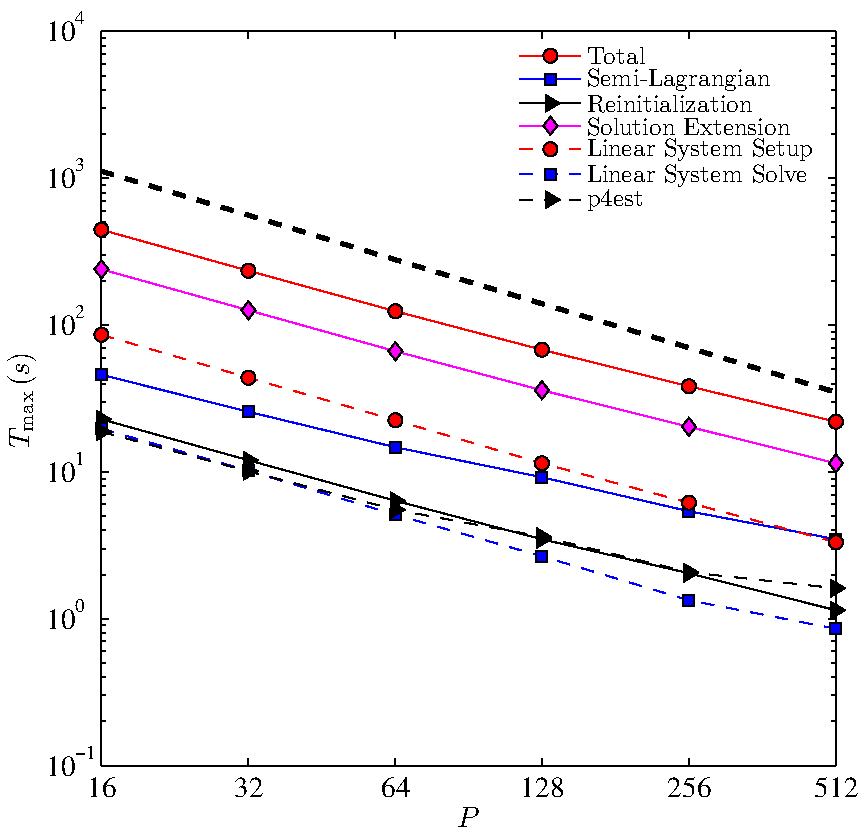
\includegraphics[width=0.45\textwidth]{figures/stefan_scaling_small.pdf}}
\subfigure[]{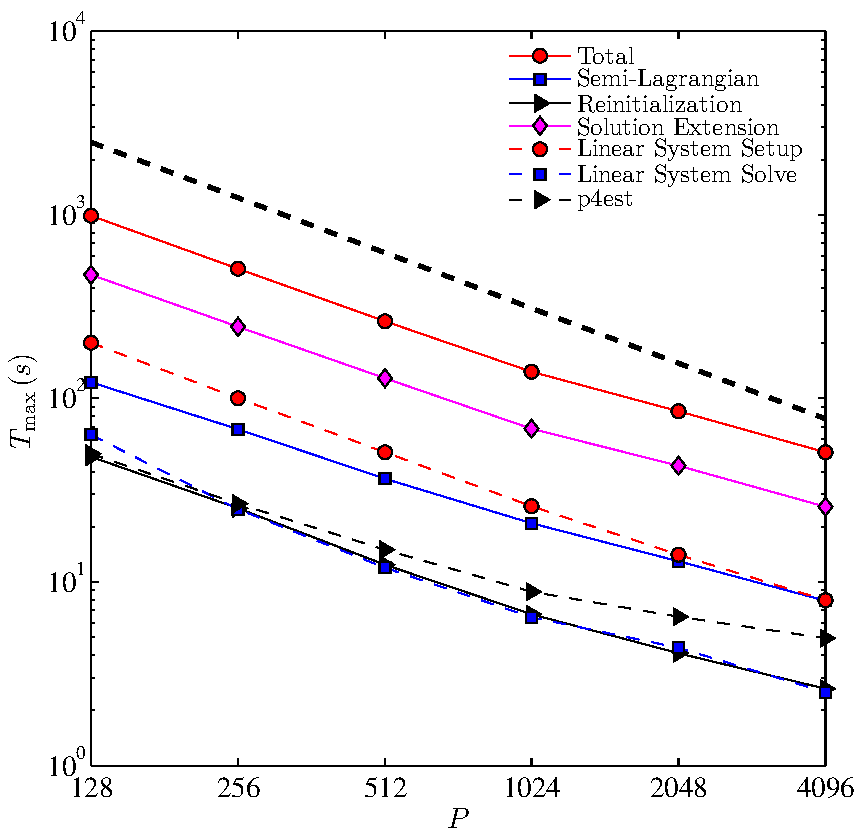
\includegraphics[width=0.45\textwidth]{figures/stefan_scaling_large.pdf}}
\caption{Scalability of the Stefan problem for small (left) and large (right) octrees with roughly 7M and 105M grid points, respectively. As expected from the scalability analysis of the individual components, we observe excellent results, illustrating the potential \mohammad{applicability?} of our solver \mohammad{algorithms?}.}
\label{fig:stefan_scaling}
\end{figure}

\subsection{Numerical experiments}
\mohammad{too many transitive statements and keyword ``choose''. Can we rephrase this?}
We now present the results from a large simulation of the Stefan problem. We choose to work with a $20\times20\times20$ macro-mesh and with level-10 octrees. We choose to define the Gibbs-Tompson anisotropy undercooling coefficients \eqref{eq:stefan_gibbs_tompson} as
\begin{align*}
\epsilon_c & = \left[ \epsilon_1 \left( 1+\alpha_1 \cos(3\theta_1) \right) + \epsilon_2 \left( 1+\alpha_2 \cos(3\theta_2) \right) \right] \kappa,\\
\epsilon_v & = 0,
\end{align*}
with $\theta_1$ the angle between the normal to the interface $\mathbf{n}$ and the x-axis in the $(x,y)$ plane, $\theta_2$ the angle between $\mathbf{n}$ and the x-axis in the $(x,z)$ plane, and
\begin{align*}
\epsilon_1 & = 2~(\sin(x)+\cos(y)+2)\cdot10^{-6}, & \epsilon_2 & = 2~(\sin(x)+\cos(z)+2)\cdot10^{-6}, \\
\alpha_1 & = \frac{1}{4}(\cos(x)+\sin(y)+2), & \alpha_2 & = \frac{1}{4}(\cos(x)+\sin(z)+2).
\end{align*}
Note that these expressions are arbitrary and lead to very varied crystal shapes \mohammad{How about: ... lead to a variety of shapes?}. The computation is initialized with twenty spherical seeds of radius $0.0015$ placed randomly in the domain. We choose $D_s=D_l=1$ and set the initial temperatures $T^0_l=-0.25$ and $T^0_s=0$.

We let the simulation run with \mohammad{How about: The simulation is ran on ...} $256$ mpi processes for $6$ hours and $30$ minutes, resulting in $396$ time iterations. Visualizations of the final iteration are presented in figures \ref{fig:stefan_grid} and \ref{fig:stefan_crystals}. The final iteration of the simulation consisted of $167$M grid points when a uniform grid with the equivalent finest resolution would lead to $8.59\cdot10^{12}$ grid points, i.e. over eight trillion grid points ! Our simulation used only $0.001948\%$ \mohammad{I think if we are going to report percentage, we should trim it to 1st digit} of the number of grid points needed for the same simulation on a uniform grid. This application demonstrates the potential of our approach.

\begin{figure}[ht!]
\begin{center}
\subfigure[]{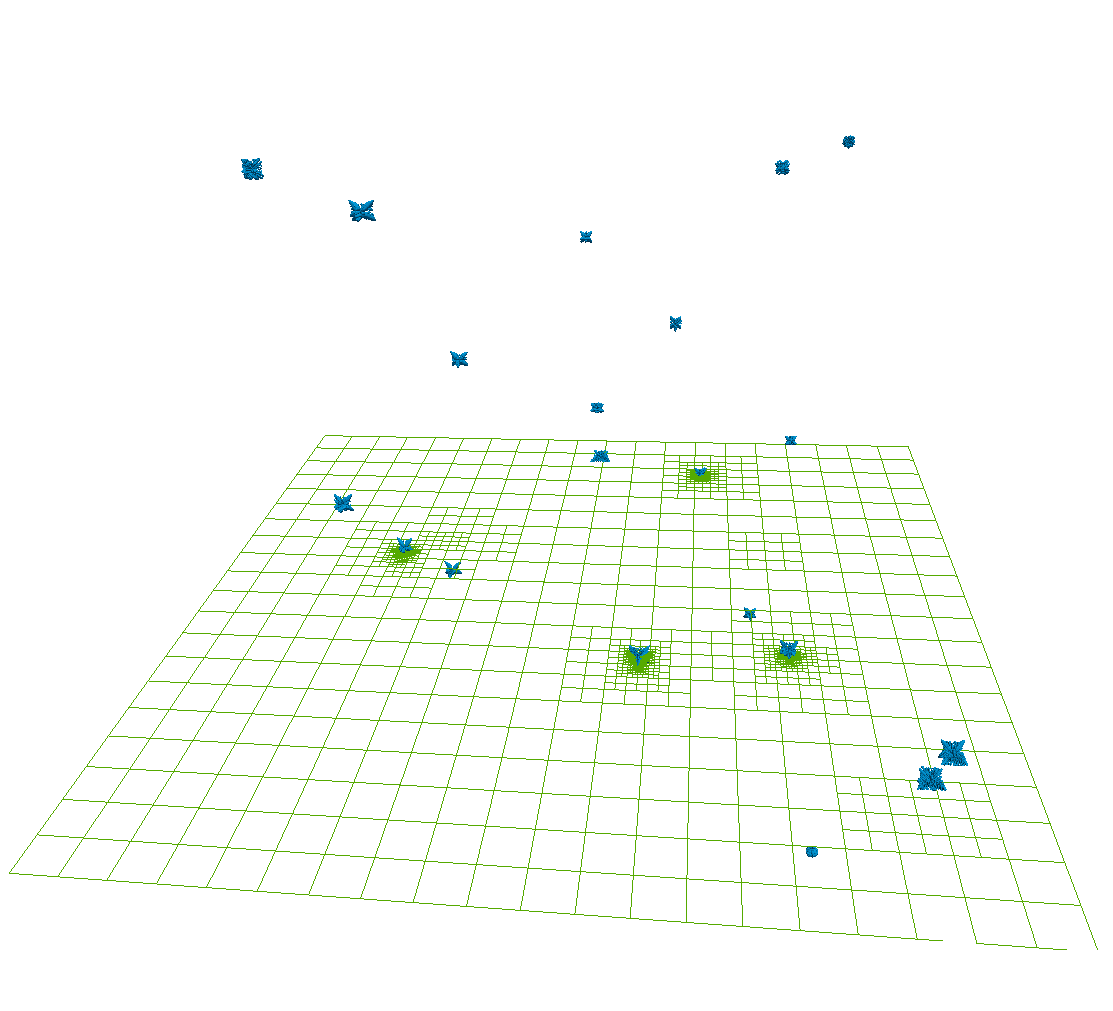
\includegraphics[width=0.45\textwidth]{figures/stefan_grid_overview.png}}
\subfigure[]{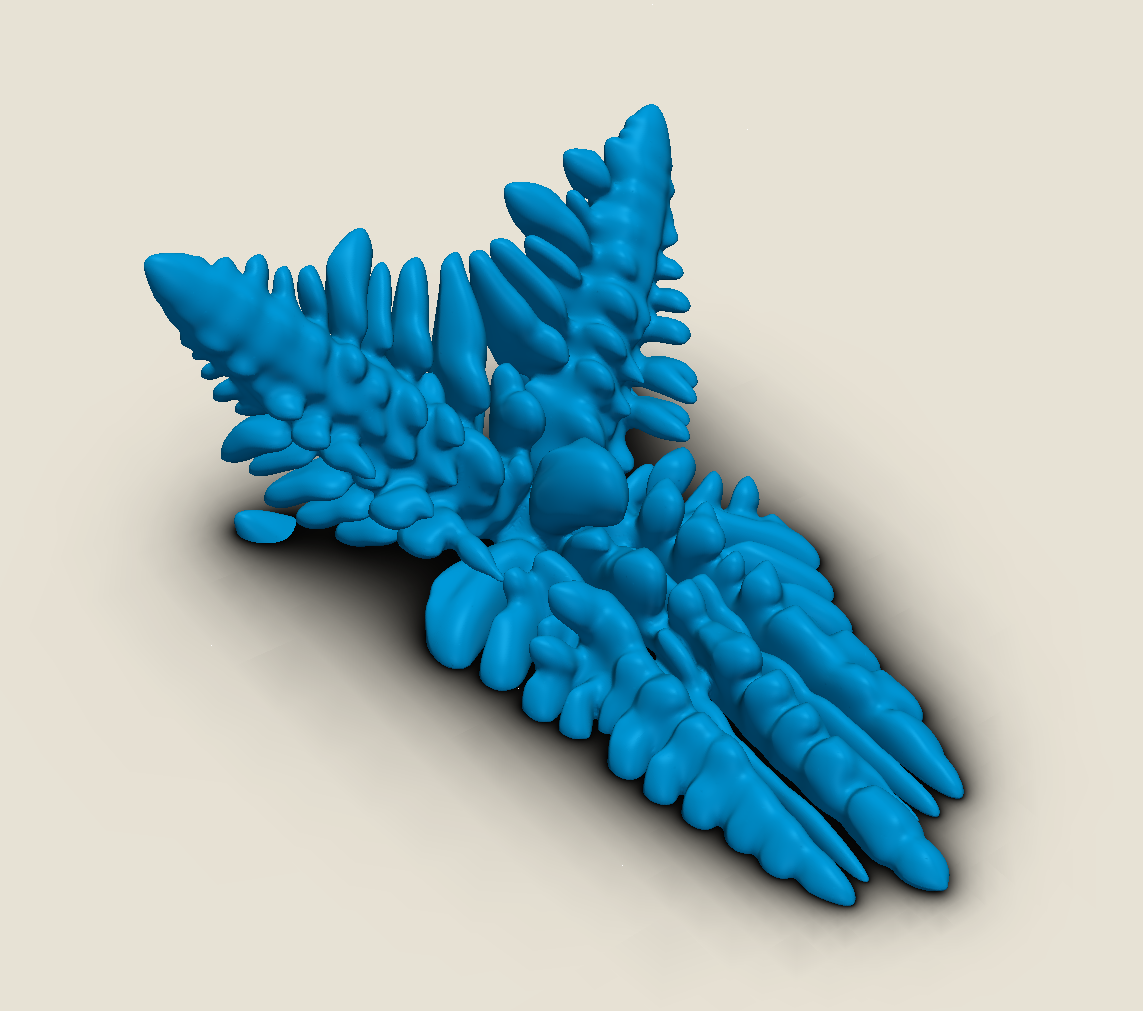
\includegraphics[width=0.45\textwidth]{figures/stefan_temperature.png}}
\subfigure[]{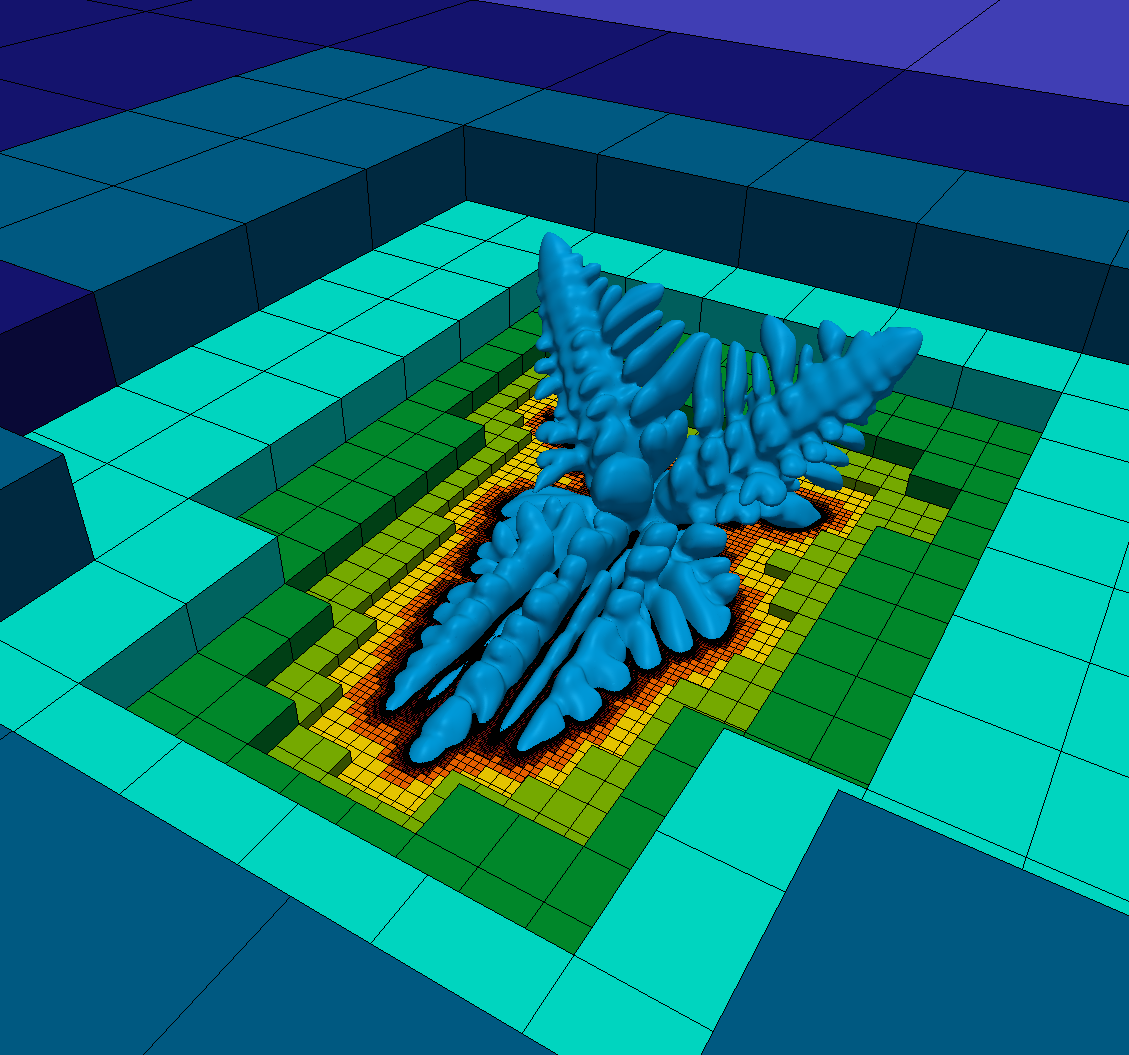
\includegraphics[width=0.45\textwidth]{figures/stefan_grid.png}}
\subfigure[]{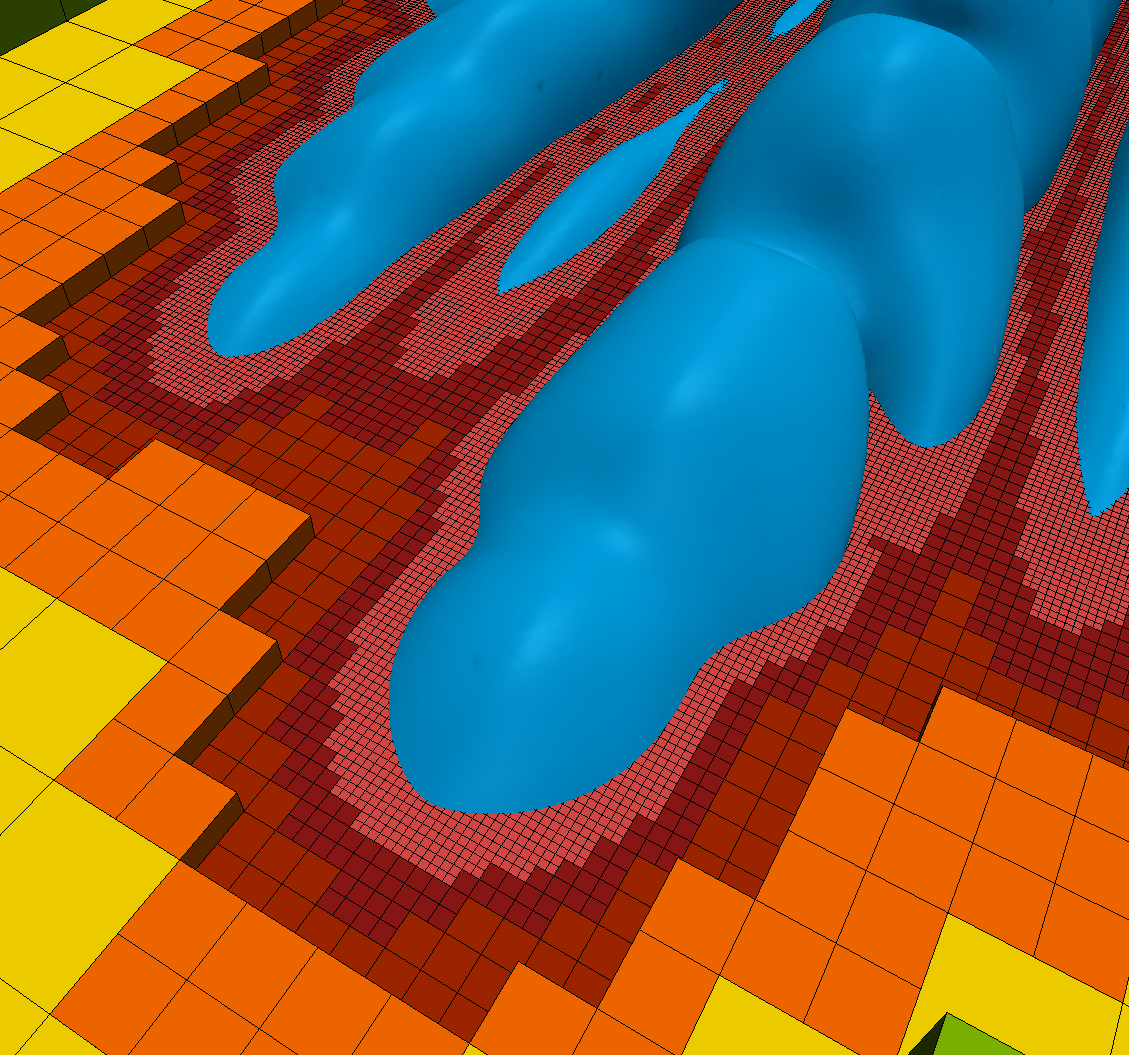
\includegraphics[width=0.45\textwidth]{figures/stefan_grid_zoom.png}}
\caption{Visualization of the computational mesh (a,b,c) and the temperature field (b) for the Stefan problem simulation.} \label{fig:stefan_grid}
\end{center}
\end{figure}

\begin{figure}[ht!]
\begin{center}
\subfigure[]{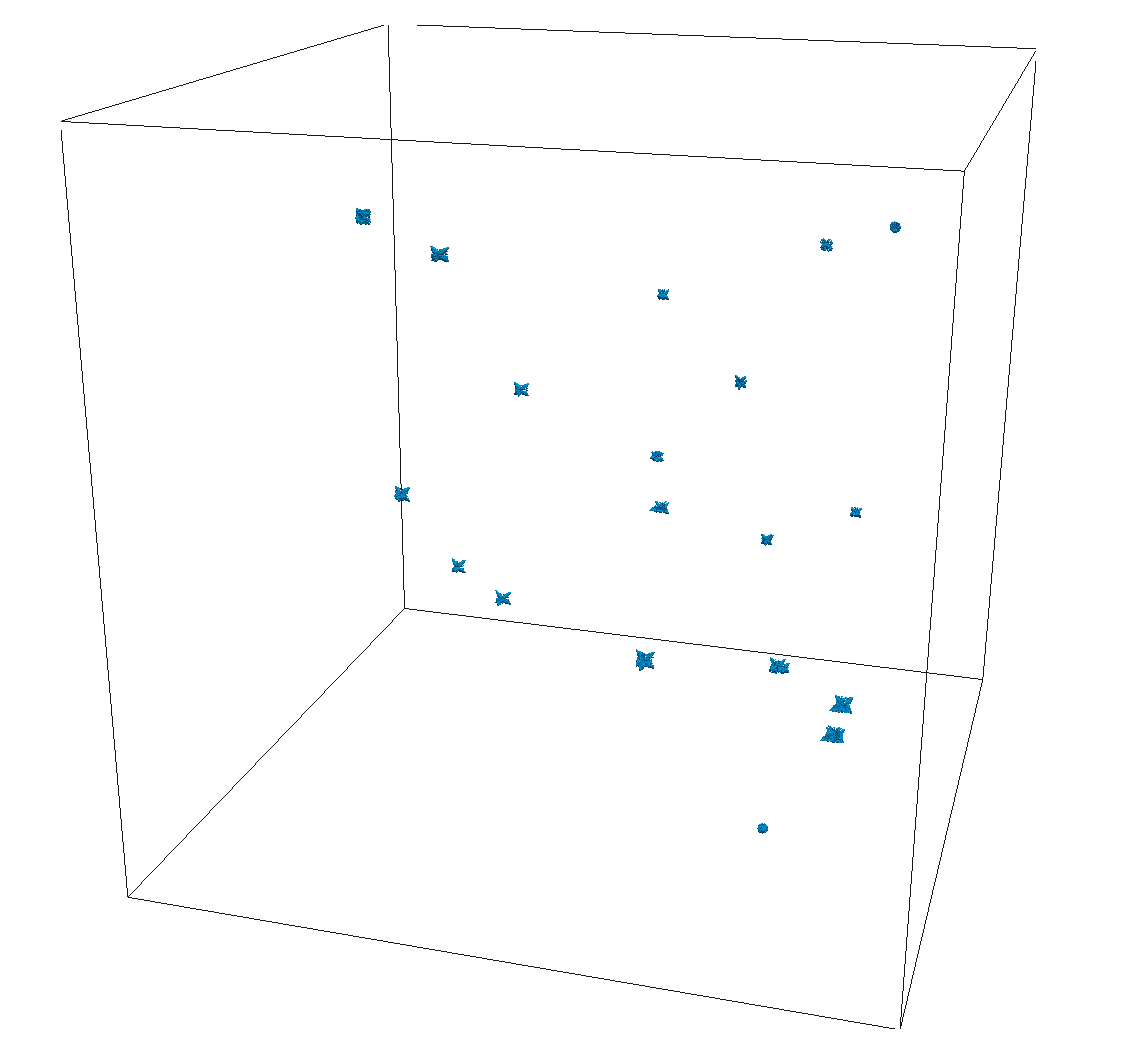
\includegraphics[width=0.45\textwidth]{figures/stefan_crystal_1.png}}
\subfigure[]{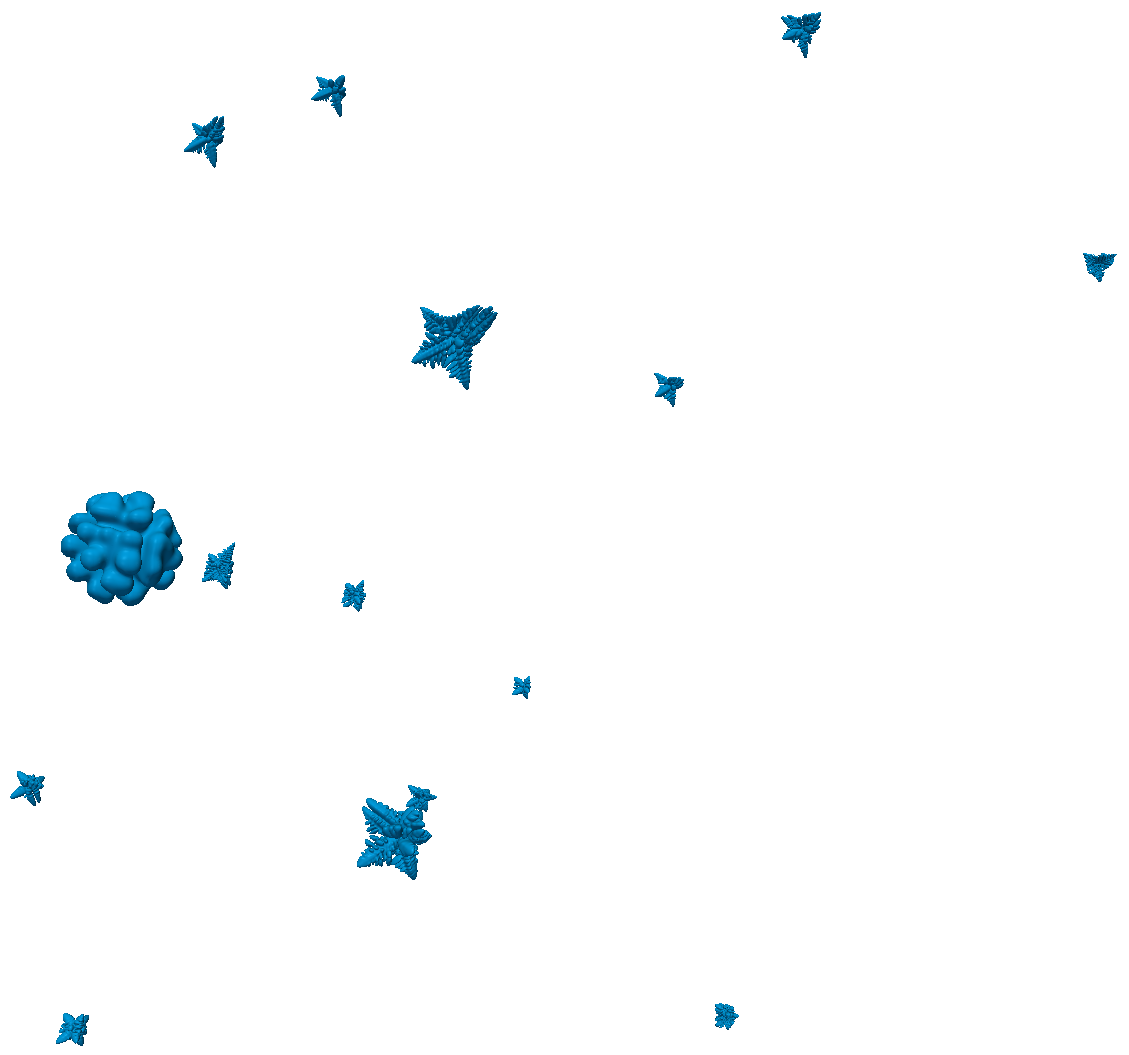
\includegraphics[width=0.45\textwidth]{figures/stefan_crystal_2.png}}
\subfigure[]{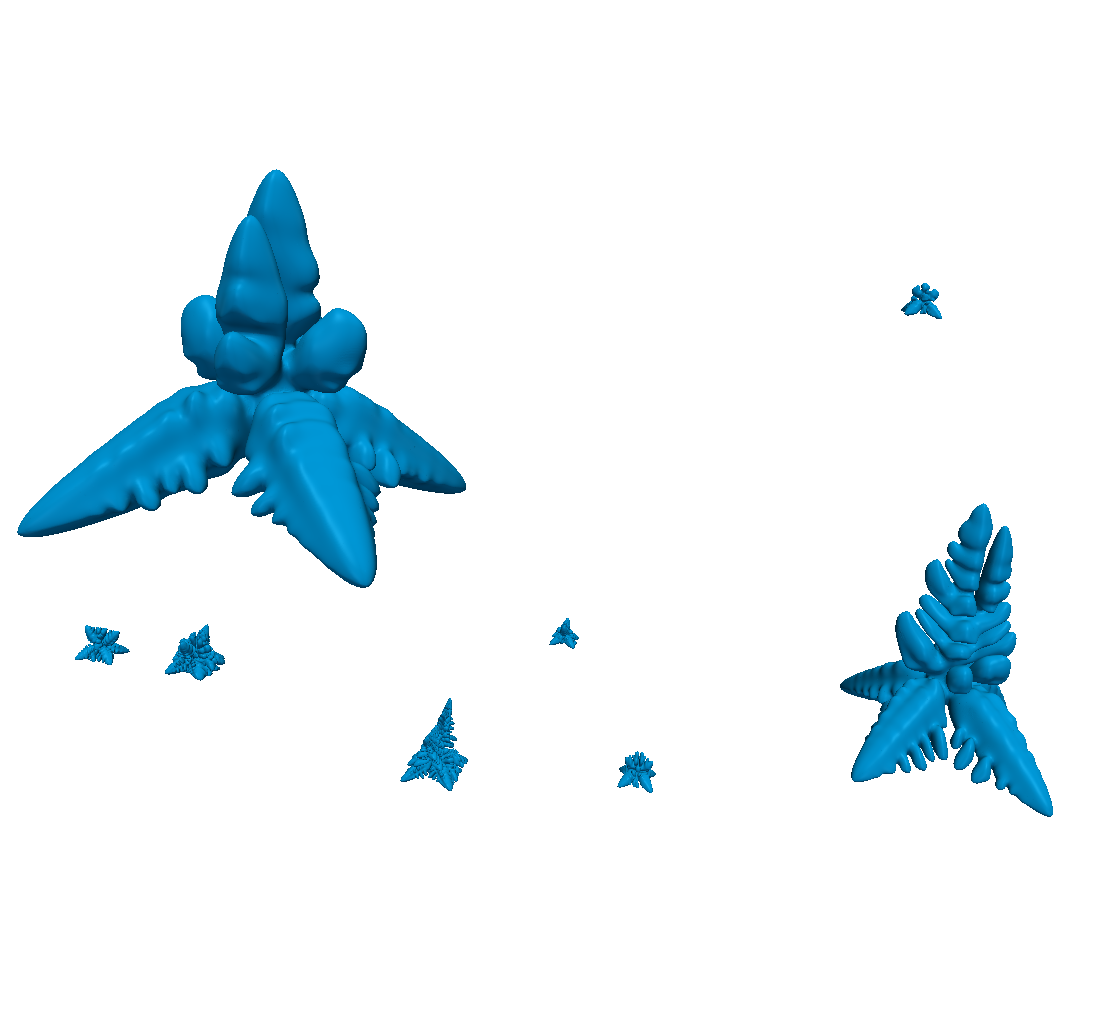
\includegraphics[width=0.45\textwidth]{figures/stefan_crystal_4.png}}
\subfigure[]{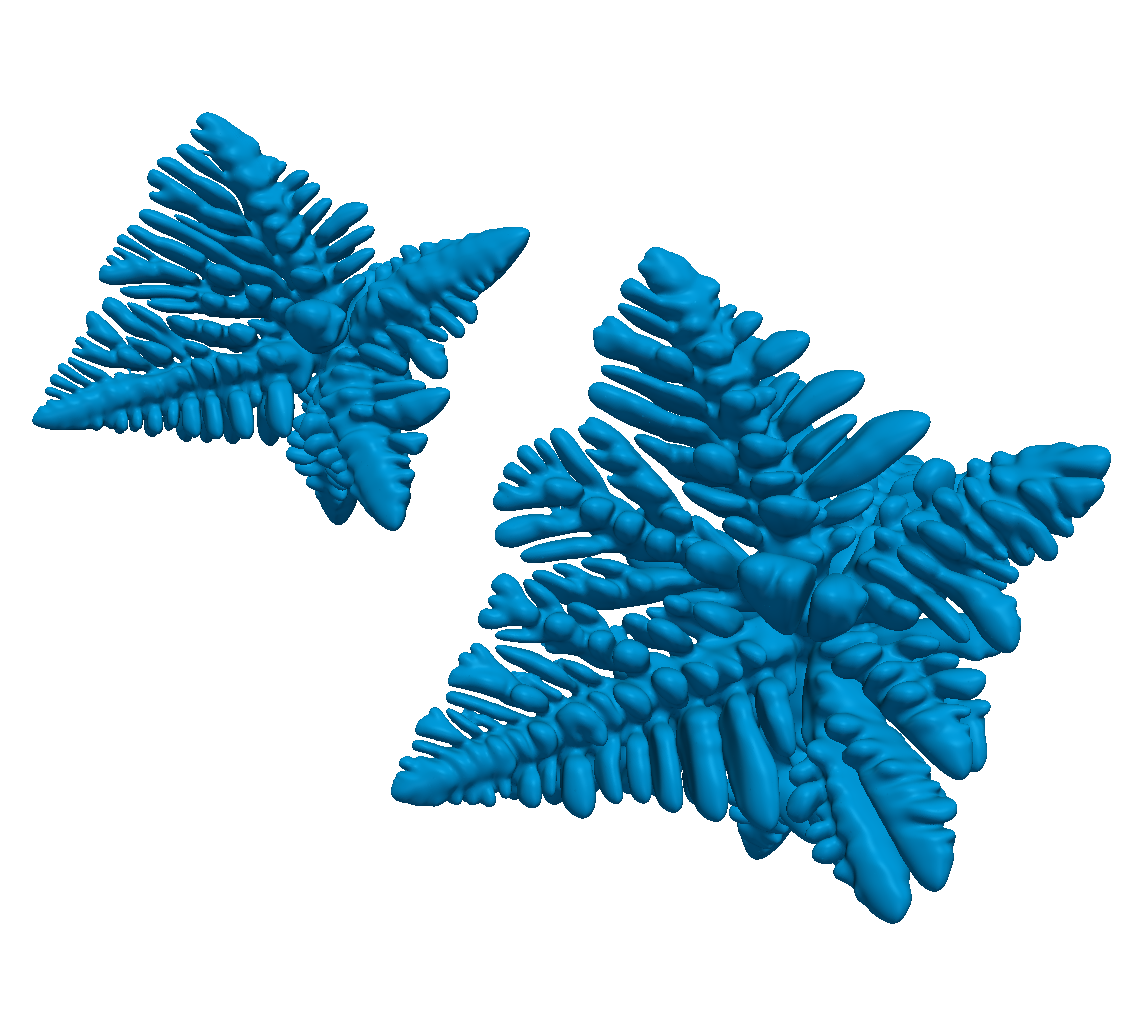
\includegraphics[width=0.45\textwidth]{figures/stefan_crystal_3.png}}
\caption{Representation of the computational domain (a) and of various crystal observed for the Stefan problem simulation.} \label{fig:stefan_crystals}
\end{center}
\end{figure}